% @Author: AnthonyKenny98
% @Date:   2020-04-04 12:27:50
% @Last Modified by:   AnthonyKenny98
% @Last Modified time: 2020-04-04 15:24:11
% @Author: AnthonyKenny98
% @Date:   2020-04-04 11:13:58
% @Last Modified by:   AnthonyKenny98
% @Last Modified time: 2020-04-04 12:09:59
% @Author: AnthonyKenny98
% @Date:   2020-02-29 17:30:44
% @Last Modified by:   AnthonyKenny98
% @Last Modified time: 2020-04-03 14:28:30
\begin{figure}[H]
\begin{center}
\begin{tabular}{cc}

    % Subfigure A
    \begin{subfigure}{0.4\textwidth}
    \begin{center}
    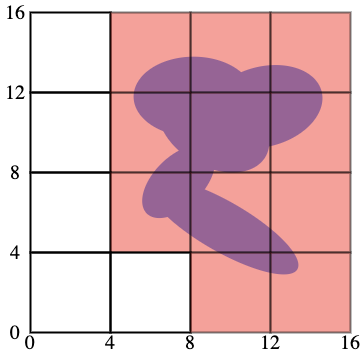
\includegraphics[width=\linewidth]{chapters/chapter2/img/motionPlanning/OGMlowres.png}
    \caption{}
    \label{subfig:OGM_A}
    \end{center}
    \end{subfigure}
    &
    % 
    % Subfigure B
    \begin{subfigure}{0.4\textwidth}
    \begin{center}
    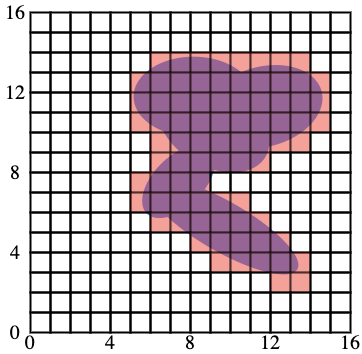
\includegraphics[width=\linewidth]{chapters/chapter2/img/motionPlanning/OGMhighres.png}
    \caption{}
    \label{subfig:OGM_B}
    \end{center}
    \end{subfigure} \\
\end{tabular}
    % Caption and Label
    \caption[Occupancy Grid Maps for $(16\times16)$ Workspace of Different Resolutions]{Comparison of Occupancy Grid Maps for $16\times16$ Workspace with Different Resolutions. Figure \ref{subfig:OGM_A} shows how an OGM with low resolution, while simpler to construct and analyse, will over-represent the obstacle density of a workspace. Figure \ref{subfig:OGM_B} shows how a higher resolution will more accurately reflect the obstacles of a workspace.}
    \label{fig:OGM}

\end{center}
\end{figure}